\chapter{Generative Models for Mechanism Synthesis}\label{ch-generative-models}
\section{Introduction}
%   Computational methods for kinematic synthesis of mechanisms for motion generation problems require input in the form of precision positions. Given the highly non-linear nature of the problem, solutions to these methods are overly sensitive to the input -- a small perturbation to even a single position of a given motion can change the topology and dimensions of the synthesized mechanisms drastically. Thus, the synthesis becomes a blind iterative process of maneuvering precision positions in the hope of finding good solutions. In this chapter, we present a deep-learning based framework which manages the uncertain user input and provides the user with a higher level control of the design process. The framework also imputes the input with missing information required by the computational algorithms. 
 
%  The approach starts by learning the probability distribution of possible linkage parameters with a deep generative modeling technique, called Variational Auto Encoder (VAE). In addition, the framework can incorporate contextual information which can be used to further condition the inputs so as to find linkages with desired properties. This context can be expressed as constraints on solution parameters, which are not directly consumable by solvers. This chapter also presents a data-driven strategy to learn such contexts, allowing for evermore flexible problem specification.  

In our quest to develop this framework, it is critical that the framework has the ability to understand salient aspects of the linkage parameters and create diverse design concepts for a given task.  This chapter presents our step in this direction by formulating a generative model of linkage parameters.

A generative model is based on generative learning principal, which does not just passively observe the events it experiences, but constructs its own perceptions about them.
For example, training a generative model for coupler curves of four-bar linkage formulates an understanding of the kind of curves a four-bar linkage can or cannot generate.
This understanding is useful in various tasks such as input denoising, modification or imputation.
Here, input imputation is defined as the process of adding the missing information in the input which is necessary for the solver to process.
Generative models encapsulate the salient information about the observed data which is essential for tasks involving recognition, representation and computational creativity.
In this work, we have used VAE~\cite{Kingma2014AutoEncodingVB} as our generative modeling framework.
The parameters of generative models are much less in number than that of the data it is trained on.
Thus, the model is forced to capture salient attributes and their variation to generate the data similar to it.
This encapsulation of salient features is utilized in tasks that require an understanding of the data.
In our case, we use it in providing the user a high-level control on manipulating different aspects of input data and to manage input uncertainties.
  
This chapter is organized as follows.
Section~\ref{sec_arch} reviews neural network architectures used in the research.
Section~\ref{sec_theory} presents the theoretical formulation of VAE.


\section{Review on Neural Network Architectures}\label{sec_arch}

\subsection{Convolutional Neural Networks}\label{subsec_deepconv}
Capturing patterns in the images is a well-researched topic; see Forsyth and Ponce~\cite{forsyth2002computer}. The computer vision literature has witnessed a vast amount of research ranging from classical computer vision approaches to deep convolutional networks. Classical computer vision approaches use hand-crafted feature extractors for capturing spatial correlations, whereas deep convolution networks learn these feature extractors from the training data.  


Convolutional Neural Networks (CNNs) are constructed to capture the spatial structure of the input~\cite{krizhevsky2012imagenet}.
CNNs consist of a set of learnable filters. In the 2D case, these filters can be represented by 2D matrices, whose coefficients are updated at each step of the training process. At the time of inference, each CNN filter is convolved around the image. A high score is reported for a strong pattern match between the filter and input. The high score gets passed on to the next layer through max pool operation.

In simple words, the output of each layer in CNN is an agglomeration of scores for various learned filters used during the convolution. This ability enables CNN to learn low-level spatial features like edges in the initial layers. As the layers go deep, the composition of simple features constitutes highly complex spatial structures depending upon the training data. 

\paragraph{Convolution Operation}
Convolutional layer use convolution operation between two entities. In the continuous case, the convolution of two functions $f$ and $g$ is given by,
\begin{equation}
    (f*g)(t) = \int_{-\infty}^{\infty} f(\tau)g(t-\tau)d\tau = \int_{-\infty}^{\infty} f(t-\tau)g(\tau)d\tau.
\end{equation}

In the discrete case, it is replaced by the sum
\begin{equation}
    (f*g)(n) = \sum_{m=-\infty}^{\infty} f(n)g(n-m) = \sum_{m=-\infty}^{\infty} f(n-m)g(m)
\end{equation}
Here, $g$ is called a kernel function. In 2D discrete case, $g$ can be represented via a 2D matrix which has support on $\{ (-M, -N), \hdots, (M, N)\}$. Then, convolution is given by
\begin{equation}\label{eq_conv2d}
    (f*g)(x, y) = \sum_{m=-M}^{M} \sum_{n=-N}^{N} f(x-n, y-m)g(m, n).
\end{equation}
Equation~\req{eq_conv2d} has a very simple geometric interpretation as shown in Fig.~\ref{fig_conv_pooling}. A 2D filter of size ($f$, $f$) is slid along the image with stride $s$. Before each sliding action, a sum is conducted and stored into an output tensor at a location governed by number of strides. The final outcome of such operations is a 2D matrix. This entire process is repeated for $k$ number of filters resulting into $k$ number of 2D matrices as shown in the figure. 
\begin{figure}
\centering
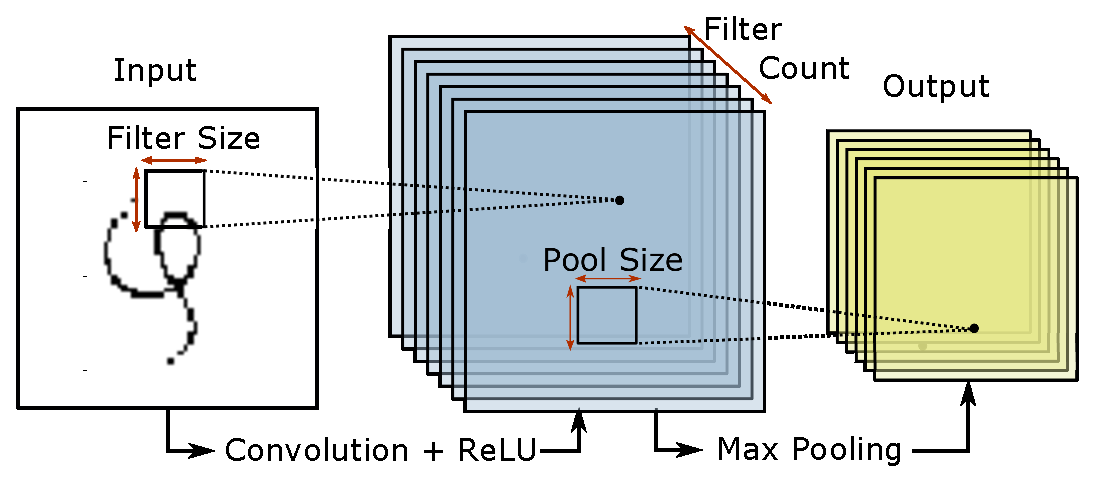
\includegraphics[width=250pt]{idetc-20/figure/fig_conv.eps}
  \caption{A filter is a 2D matrix whose coefficients are the learnable parameters of the convolution network. During convolution, each of such filter it is convolved on the input followed by nonlinear ReLU activation resulting in $k$ such 2D matrices as shown by the middle entity. Next, the output is max pooled to formulate the output to be passed on to the next layer.}
\label{fig_conv_pooling}
\end{figure}
In CNN, the learning parameters are the coefficients of kernel matrices. These coefficients are updated via the Backpropagation algorithm in a stochastic gradient descent method of optimization. For more details; please see see~\cite{bottou2010large},~\cite{rumelhart1986learning}.

\subsection{CNN-VAE Architecture for Image Representation of Coupler Curves}
The input to the encoder is a $64\times64$ image. This input is fed to three stacks of convolutional-MaxPooling layers. The output of the convolutional layer is first passed through ReLU activation before it can be max pooled. Max pooling layer passes the highest activation in the filter window to the next layer. The hyper-parameters for each layer are given in Table~\ref{tab_encoder_paras}. After three such layers, the output is flattened into a single vector, which then is connected to a single fully connected layer which outputs two vectors representing $\mu$ and $\log\sigma$ of 50 dimensions each. Vector $z$ is obtained by sampling a multivariate Gaussian distribution with mean $\mu$ and standard deviation $\sigma$. This vector is passed to the generative model as an input.

\begin{table*}
  \caption{Recognition Network Architecture}
\centering
\label{tab_encoder_paras}
\begin{tabular}{cccccc}
\hline
  Layer & Filter Count & Filter Size & Stride & Output Shape & Activation\\
\hline
  Convolution 1 & 32 & (11, 11) & (1,1) & (64, 64, 32) & ReLU \\
  Max Pooling 1 & - & (2,2) & (2,2) & (32, 32, 32) & -  \\
  Convolution 2 & 64 & (5, 5) & (1,1) & (32, 32, 32) & ReLU   \\
  Max Pooling 2 & - & (2,2) & (2,2) & (16, 16, 64) & - \\
  Convolution 3 & 128 & (3, 3) & (1,1) & (16, 16, 128) & ReLU   \\
  Max Pooling 3 & - & (2,2) & (2,2) & (8, 8, 128) & - \\
  Flatten 1 & - & - & - & 8192 & - \\
  Fully Connected & - & - & - & 100 & - \\
  Split & - & - & - & (2, 50) & (-, exponential) \\ \hline 
\end{tabular}
\end{table*}



The generative model architecture is composed of transpose-convolution layers to finally output a tensor similar to that of image. The architecture and hyper-parameters are given in Table~\ref{tab_decoder_paras}.

\begin{table*}
  \caption{Generative Network Architecture}
\centering
\label{tab_decoder_paras}
\begin{tabular}{cccccc}
\hline
  Layer & Filter Count & Filter Size & Stride & Output Shape & Activation\\
\hline
  Fully Connected & - & - & - & 1024 & ReLU \\
  Reshape & - & - & - & (8, 8, 16) & - \\
  Transpose Convolution 1 & 128 & (3, 3) & (2,2) & (16, 16, 128) & ReLU   \\
  Transpose Convolution 2 & 64 & (5, 5) & (2,2) & (32, 32, 64) & ReLU   \\
  Transpose Convolution 3 & 32 & (11, 11) & (2,2) & (64, 64, 32) & ReLU   \\
  Transpose Convolution 3 & 1 & (3, 3) & (1,1) & (64, 64, 1) & Sigmoid   \\
\hline
\end{tabular}
\end{table*}


\section{Theory of Variational Auto Encoders (VAE)}\label{sec_theory}
\begin{figure}
\centering
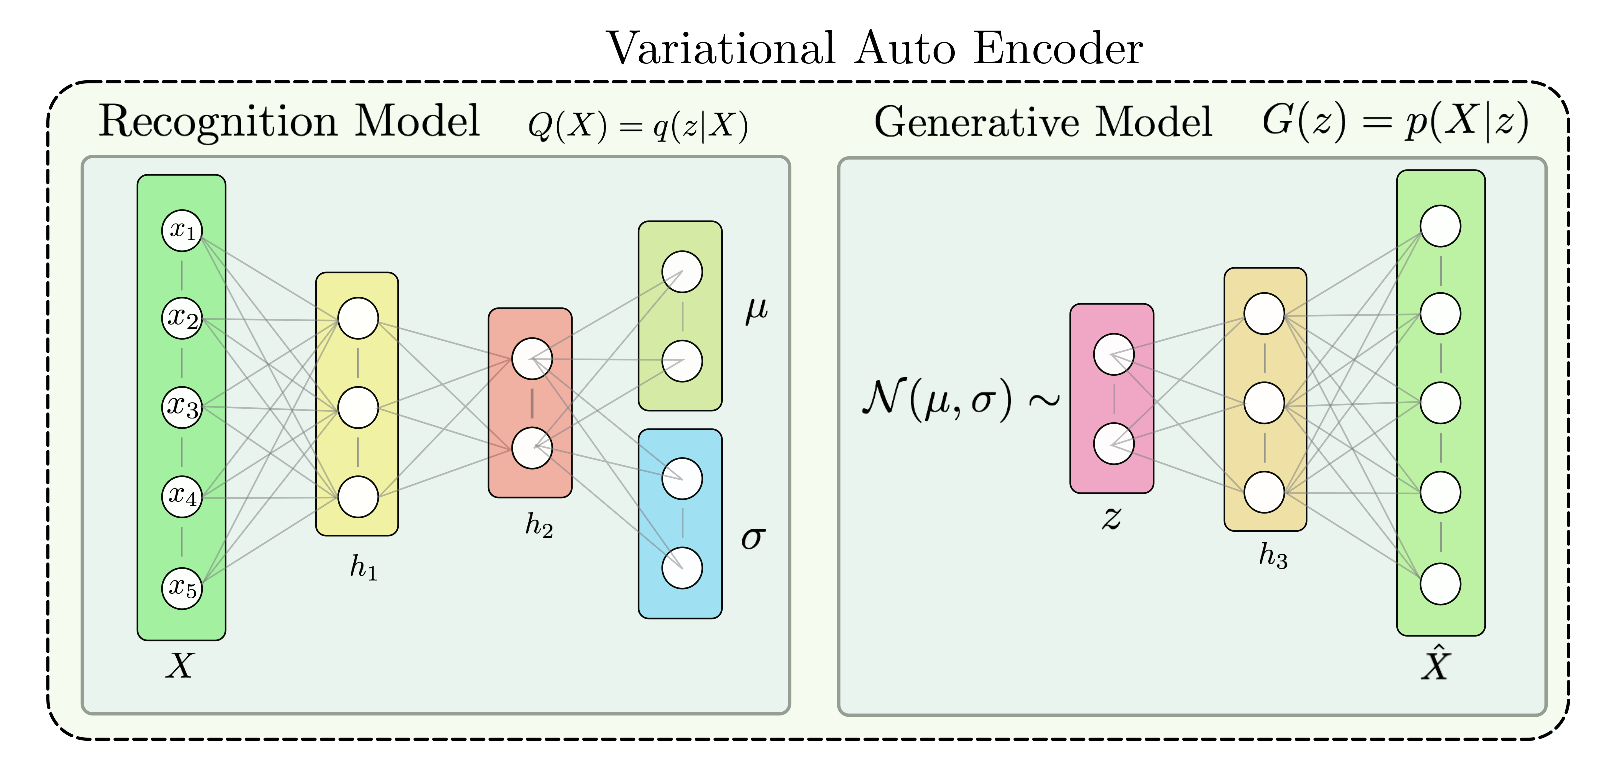
\includegraphics[width=300pt]{jmd-19/figure/fig_vae.eps}
  \caption{Recognition Model encodes the observed data $X$ into probabilistic latent coding $z$ of dimension much smaller than $x$. In this case, we assume a multivariate Gaussian distribution for $z$. Generative Model takes samples from this distribution to generate output $\hat{x}$.}
\label{vae_arch}
\end{figure}

\begin{figure*}
\centering
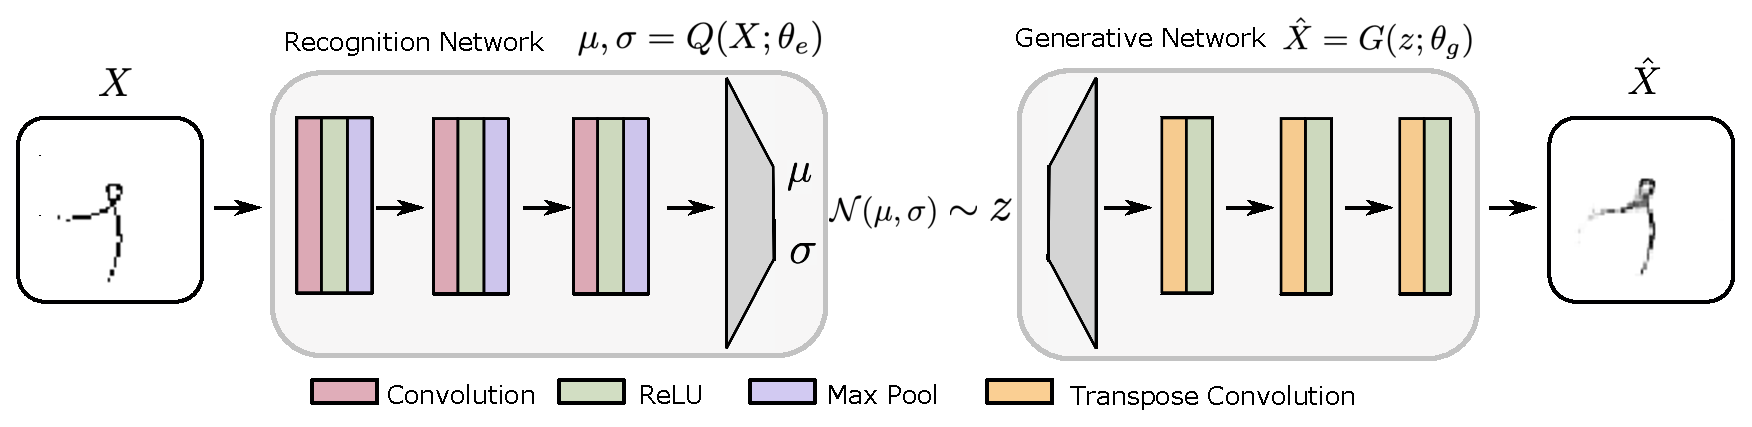
\includegraphics[width=\textwidth]{idetc-20/figure/fig_conv_vae.eps}
  \caption{CNN-VAE Architecture for Image Representation of Coupler Curves. For encoder, each hidden layer consists of convolution, ReLU and max pooling operation. For decoder each hidden layer consists of transposed-convolution and relu operation.}
\label{fig_conv_vae}
\end{figure*}

VAE~\cite{Kingma2014AutoEncodingVB} is a neural network architecture that learns to approximate the true distribution of an observed data $x$.
In this work, different models of VAE are trained to learn different observed data, thus $x$ can represent different quantities for different VAEs.
Depending upon the quantity that $x$ represents, $x$ can have different dimensions.
For example, if a VAE is trained on the coupler path dataset, then $x$ represents coupler paths and will be denoted by \ac{x_path_vector}\footnote{When the path is represented as a sequence of points} or \ac{x_path_im}\footnote{When the path is represented as images}.
Whereas, if VAE is trained on coupler motions or four-bar linkage parameters, then $x$ would represent coupler motions (\ac{x_motion_vector}) and four-bar linkages (\ac{x_fourbar}), respectively. $x$ can be a set of points or tensor representing images.

Figure~\ref{vae_arch} shows a representative architecture of VAE. In this architecture, the Recognition Model encodes the data into the probability distribution of latent variables, while the Generative Model is responsible for generating new data or reproducing trained data.
In the middle of this figure, there is feature space encoded by the variable $z$, which seeks to capture the essence of the input data.  
However, as opposed to Auto Encoder architecture in which $z$ is a discrete variable, in the VAE, the $z$ is determined via a probability density function.

Let us assume that the $d$ dimensional data $x$ is highly structured and occupies a much smaller $k$ dimensional space.
We know that a $k$ dimensional unit Gaussian distribution can be mapped into any $k$-dimensional distribution through a nonlinear mapping.
In other words, it can be said that the data $x$ is generated by some natural process
that maps a $k$ dimensional variable $z$ to $d$-dimensional variable $x$.
We try to mimic this process with an unknown parametric generative model based on hidden variable $z$, given that probability distribution of $z$ is unit Gaussian, .
\begin{eqnarray}
pr(z) = \mathcal{N}(0, 1)\label{pz},\\
  x = G(z; \theta_g)\label{eq_G},
\end{eqnarray}
where $\theta_g$ are weight parameters of the neural network that acts as the generative model.
The variable $z$ is called the latent variable, which contains salient information of the observed variable $x$.
We would like to infer salient attributes $z$ based on observed $x$, which can be expressed by conditional probability $pr(z|x)$
\begin{equation}
pr(z|x) = \frac{pr(x|z)pr(z)}{pr(x)},
\end{equation}
where the abbreviation $pr(A)$ represents probability of variable A.
Unfortunately, computing probability of $x$ (i.e., $pr(x)$) is usually intractable. As it involves computing the integral $\int
pr(x|z)pr(z)dz.$
However, we can apply variational inference~\cite{blei2017variational} to estimate the joint probability distribution $pr(z|x)$.
We approximate $pr(z|x)$ by a tractable distribution $q(z|x)$, which we define such that it can be computed by a neural network $Q$.
\begin{eqnarray}\label{eq_Q}
\mu, \sigma = Q(x; \theta_e),\\
  q(z|x) = \mathcal{N}(\mu, \sigma)
\end{eqnarray}
Here, $\mathcal{N}(\mu, \sigma)$ is a multivariate Gaussian distribution function with mean $\mu$ and variance $\sigma$.
Now, we want to find parameters of Recognition Model $Q(x)$ that predict the distribution $q(z|x)$ such that it is very similar to $pr(z|x)$. Then, we can use it to perform approximate inference of the intractable distribution.

The objective is to find parameters $\theta_g, \theta_e $ of $G(z)$ and $Q(x)$ respectively such that our model generates samples as close as true observed distribution and distribution $q(z|x)$ is as close as true distribution $p(z)$.
This is achieved by training the neural network models for maximizing the lower bound of the marginal likelihood (\ac{elbo_loss}), which is given by,
\begin{equation}
  \mathcal{L_{\text{ELBO}}} = \mathbb{E}_{Q(z|x^{i}; \theta_e)}[(\log(p(x^{i}|z))) - D_{KL}(Q(z|x^{i}; \theta_e)||p(z))]  \\
\end{equation}
Here, the first term on RHS represents reconstruction likelihood and the second term is called Kullback-Leibler divergence (KL divergence)~\cite{kullback1951} which ensures that our learned distribution $Q(z|x;\theta_e)$ is similar to the true prior distribution $p(z)$.
Since we assume that $p(z)$ is a Gaussian distribution, the lower bound of marginal likelihood becomes,
\begin{equation}
   \mathcal{L_{\text{ELBO}}}^{(x^i)} = - (\hat{x}^i-x^i)^2 - (\sum_i^{k} {\sigma_i}^2 + {\mu_i}^2 - \log(\sigma_i) - 1) \\
\end{equation}

The training objective is given by,
\begin{equation}
 \argminA_{\theta_e, \theta_g} ( - \mathcal{L_{\text{ELBO}}})
\end{equation}

For further details please see \cite{Kingma2014AutoEncodingVB}. The training objecting maximizes the lower bound of marginal likelihood


Once, entire VAE is trained, the recognition model and generative model can be used separately or together depending upon the application. In what follows, we describe the details of the Recognition and the Generator Models.

\section{Recognition Model}

The architecture shown in Fig.~\ref{vae_arch} consists of a recognition model, which is an ANN.
The inputs are passed through dropout~\cite{srivastava2014Dropout}, which randomly skips a connection between input and the first hidden layer with a probability of 0.1.
This small amount of uncertainty in the input helps in learning robust patterns present in the input.
The Recognition model is comprised of hidden layers, which finally produce two $z_{dim}$ dimensional vectors representing mean and variance of latent attribute $z$.
The hidden layers can be convolutional layers or fully connected layers depending upon the nature of observed data.
Convolutional layers are often the preferred choice when dealing with images. This is due to the nature of convolution operation which connects only the neighboring neurons to capture the local pattern. 

The Output of the Recognition model is a multivariate probability distribution of the latent variable, which captures the salient attributes of the data.
Random samples drawn from this distribution are passed to the Generator network. In the case of training via the Back-Propagation algorithm, gradients are passed from generator to recognition model by the means of Reparameterization trick~\cite{Kingma2014AutoEncodingVB}.
Recognition model effectively captures the approximate posterior inference $(pr(z|x)$ of the input data and thus can be used for tasks such as recognition, denoising, representation and visualization purposes.

\section{Generator Model}
Parameters of this neural network are learned to map a latent vector to a reconstruction, which would exhibit similar latent attributes if passed through the recognition network.
Thus, the generative model can generate data whose probability distribution is similar to that of training data.
The architecture of this model starts with an input layer that receives the latent vector and passes through single or multiple layers of neurons culminating into the original size of the observed data.
The middle layers can be deconvolutional or fully connected layers that upscale the input they receive from the previous layer.

\section{Variants of VAE}
\paragraph{Denoising VAE}
VAE networks can be used to remove noise from input data.
This is done by adding noise to the input data while training.
However, the generator is forced to produce original noise-free samples by defining the reconstruction loss between the reconstructed image and the original noise-free image.
This forces the recognition network to encode robust features from the data.


\paragraph{Conditional VAE}\label{condi_vae}
Until now, we have seen VAE with unsupervised learning architectures, i.e., which requires unlabeled data for training.
\ac{cvae} is trained to learn the conditional distribution of an observed variable with respect to an explicitly observed property (or, label) $y$.
This is achieved by small modifications in the aforementioned VAE architecture.
Instead of only providing with observed data, the recognition network accepts concatenated input of $x$ and $y$.
Moreover, the generator also receives a concatenated input of $z$ and $y$.
This grants \ac{cvae} additional information for the variational inference task.
This can be used to generate samples that are highly associated with the given $y$ at the time of generation.
